% "Станет проще"

\documentclass[a4paper,12pt]{article} % тип документа

% report, book

%  Русский язык
\usepackage{ucs}
%\usepackage[T2A]{fontenc}			% кодировка
%\usepackage[utf8]{inputenc}			% кодировка исходного текста
\usepackage[utf8x]{inputenc}
\usepackage[english,russian]{babel}
%\usepackage{cmap}



\usepackage{graphicx}
\usepackage[english,russian]{babel}	% локализация и переносы



\usepackage[left=30mm, top=20mm, right=20mm, bottom=40mm, nohead, nofoot]{geometry}
% Математика
\usepackage{amsmath,amsfonts,amssymb,amsthm,mathtools}
\usepackage{csvsimple}
\usepackage{multirow}


\usepackage{wasysym}
\usepackage{subcaption}
\usepackage{gensymb}
\usepackage{verbatim}
\usepackage[hidelinks]{hyperref}
\usepackage{float}
\usepackage{enumerate}
\usepackage{wrapfig}
\usepackage{listings} %написание кода
%\usepackage{times} %шрифт
\usepackage{textcomp}


\usepackage[dvipsnames]{xcolor}
\usepackage{verbatim} %comments

%Заговолок



\graphicspath{ {img/} }


\begin{titlepage}
\author{Соловьянов Михаил}
\title{Диплом \\ \LARGE{«Разработка аналоговой электроники беззондовой измерительной системы на чипе для тестирования оксидов гафния
»\\ M04-906}}
\date{\today}
\end{titlepage}



\begin{document} % начало документа

\tableofcontents
\addcontentsline{toc}{section}{.}
\newpage



\section{Вступление и актуальность темы исследования}


Данная работа посвящена разработке аналоговых компонентов для АЦП источника измерителя чипа. Последний должен  стать инструментом для высокоскоростного  анализа всех видов энергоэффективной памяти, разрабатываемой в ЦКП МФТИ, а также некоторых других его аналоговых компонентов. Чип тестовая станция для тестирования инновационных энергоэффективных видов памяти[1][2][3] позволит оценивать быстродействие готовых массивов различной памяти, что невозможно на открытой зондовой станции, которая находиться в распоряжении исследовательских лабораторий. Помещение тестирующей аппаратуры прямо «на чип» позволяет избежать проблем, связанных с паразитными параметрами зондовых станций, что дает возможность изучать высокочастотные характеристики памяти, а также позволило бы автоматизировать процесс изучения качества выращенной памяти.



\begin{figure}[H]
    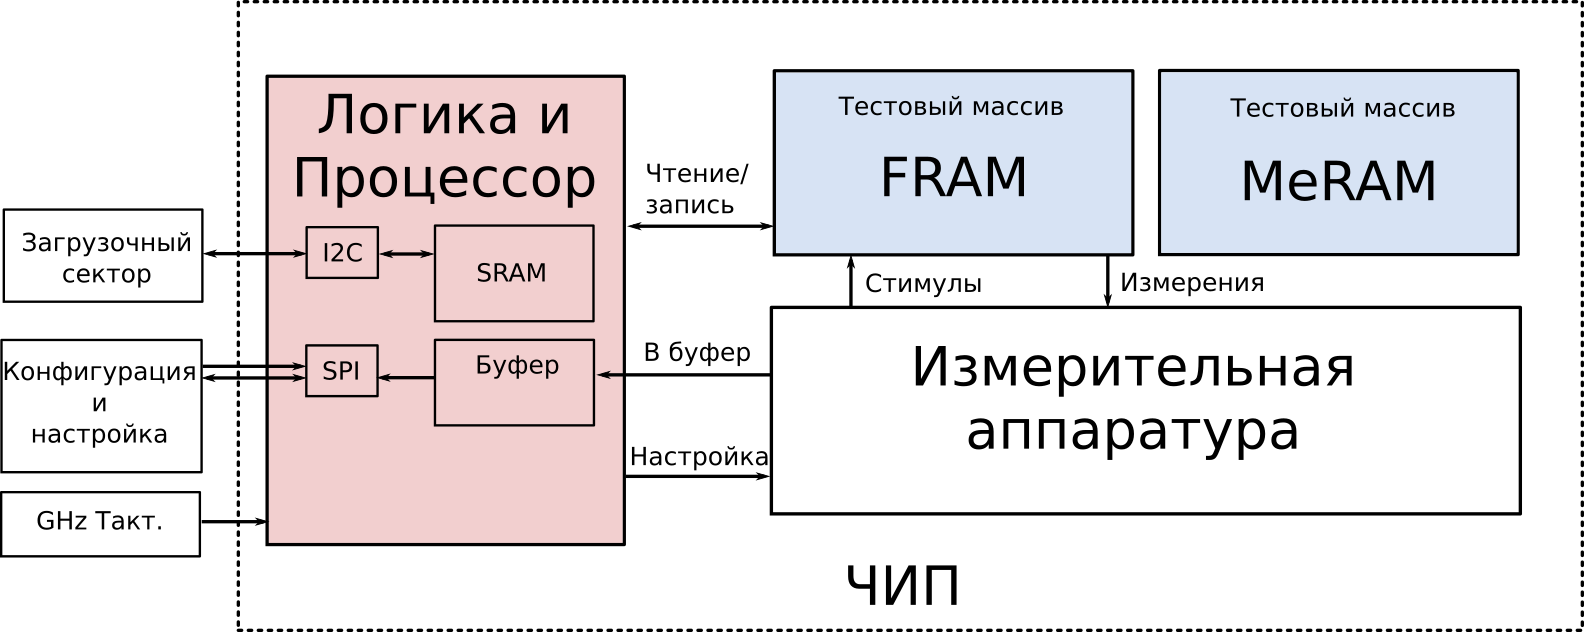
\includegraphics[width=\textwidth]{top_ru.png}
    \caption{Общая принципиальная схема}
    \label{pic:top_ru}
\end{figure}

Примерное устройство чипа представлено на рисунке и предполагает контроль/измерение нескольких ядер различной памяти, а также анализаторов отклика с возможностью подключать их как к интересующим нас столбцам выбранного стека, так и к индивидуальным ячейкам. Проект чипа покрывает спектр измерений ячеек, схожий с возможностями тестовой станции B1500A.

\section{Обзор литературы}

В первую очередь, нужно сказать, что похожие по сути проекты уже существуют и были реализованы, но без специфики оксидов изготавливаемых группой лабораторий в ЦКП МФТИ, а так же без радиационно стойких техпроцессов, что вносит свои особенности. Самой полной работой по этой части можно считать работу \cite{FRAM}. Однако, исследуемый чип предлагает решение на концептуально новых материалах, а также на достаточно больших частотах измерений. Подробно о характеристиках чипа в части [insert]. Также сравнивая направленность работ необходимо отметить, что в работе [insert], отсутствовал встроенный процессор способный выполнять сложные тесты и сохраняя результаты во внутренний буфер. Также разрабатываемый чип нацелен в первую очередь на быстрый захват выборки напряжений и токов во времени.

\section{Ход разработки}

\begin{figure}[H]
    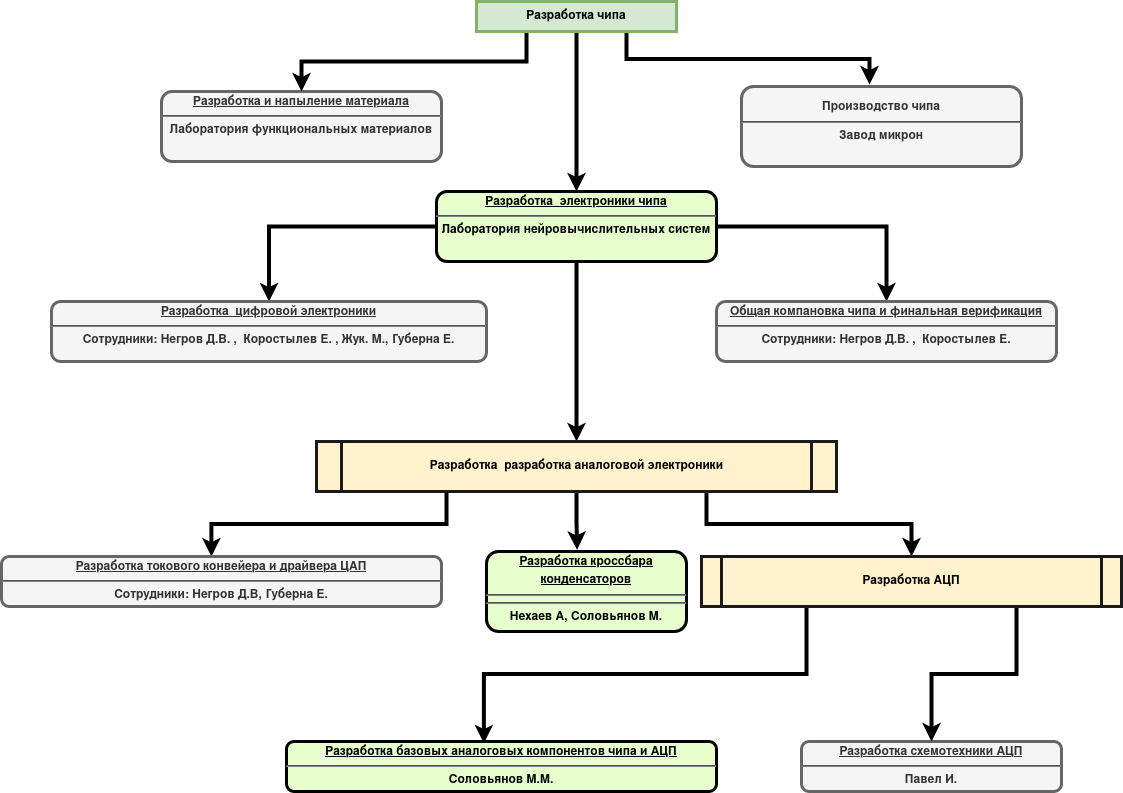
\includegraphics[width=\textwidth]{struct.png}
    \caption{Иерархия разработки}
    \label{pic:struct}
\end{figure}




Процесс разработки данного проекта  можно разделить на две фундаментальных части: Цифровую и аналоговую. Как видно из общей схемы чипа, цифровая (на рисунке красная) часть чипа проектируется на языках описания цифровой логики и выполняет задачи управления аналоговыми интерфейсами, разработка которых и описана в данной работе. Аналоговый интерфейс состоит из  двух больших частей: измерительных блоков и вспомогательной электроники. Измерительные блоки это АЦП и ЦАП, а вспомогательная электроника это система ключей для адресации измерительной аппаратуры к индивидуальным ячейкам, температурно независимые источники тока, референсы постоянных напряжений и цепи, компенсации ошибок усилителя. Каждый из этих компонентов будут рассмотрены отдельно. Так же хочется заметить что не над всеми компонентами работал я.Общая схема АЦП и ЦАП, а также система переключателей для адресации к устройствам были созданы двумя моими коллегами. Лично за мной осталась большая часть блоков применяемых для создания АЦП, такие, как компараторы, усилители, ключи и прочее. Однако рассматривать нашу работу отдельно не представляется возможным, ибо мы работали над одной задачей в условиях постоянного взаимодействия.



\subsection{Общая схема источника - измерителя}


Общая схема источника измерителя представлена ниже. Всего на чипе расположено два таких блока. Каждый из них подключается к своей обкладке конденсатора, и позволяет подавать напряжения, измерять напряжения, и протекающий через источник ток. Получается на один блок приходится один низкоимпедансный ЦАП и два АЦП для измерения тока и напряжения соответственно. Итого на измерительную часть чипа приходится 4 АЦП и 2 низкоимпедансных ЦАП.





\subsection{Техническое задание для  источника - измерителя}

\subsection{Обзор работы конвейерного АЦП (pipeline ADC)}

В основу этой работы легла разработка компонентов для создания быстродействующего конвейерного АЦП. Данная глава содержит краткое описание принципов его работы, чтобы дать обоснование поставленным к разработке требованиям по частоте и степени усиления.


\begin{figure}[H]
    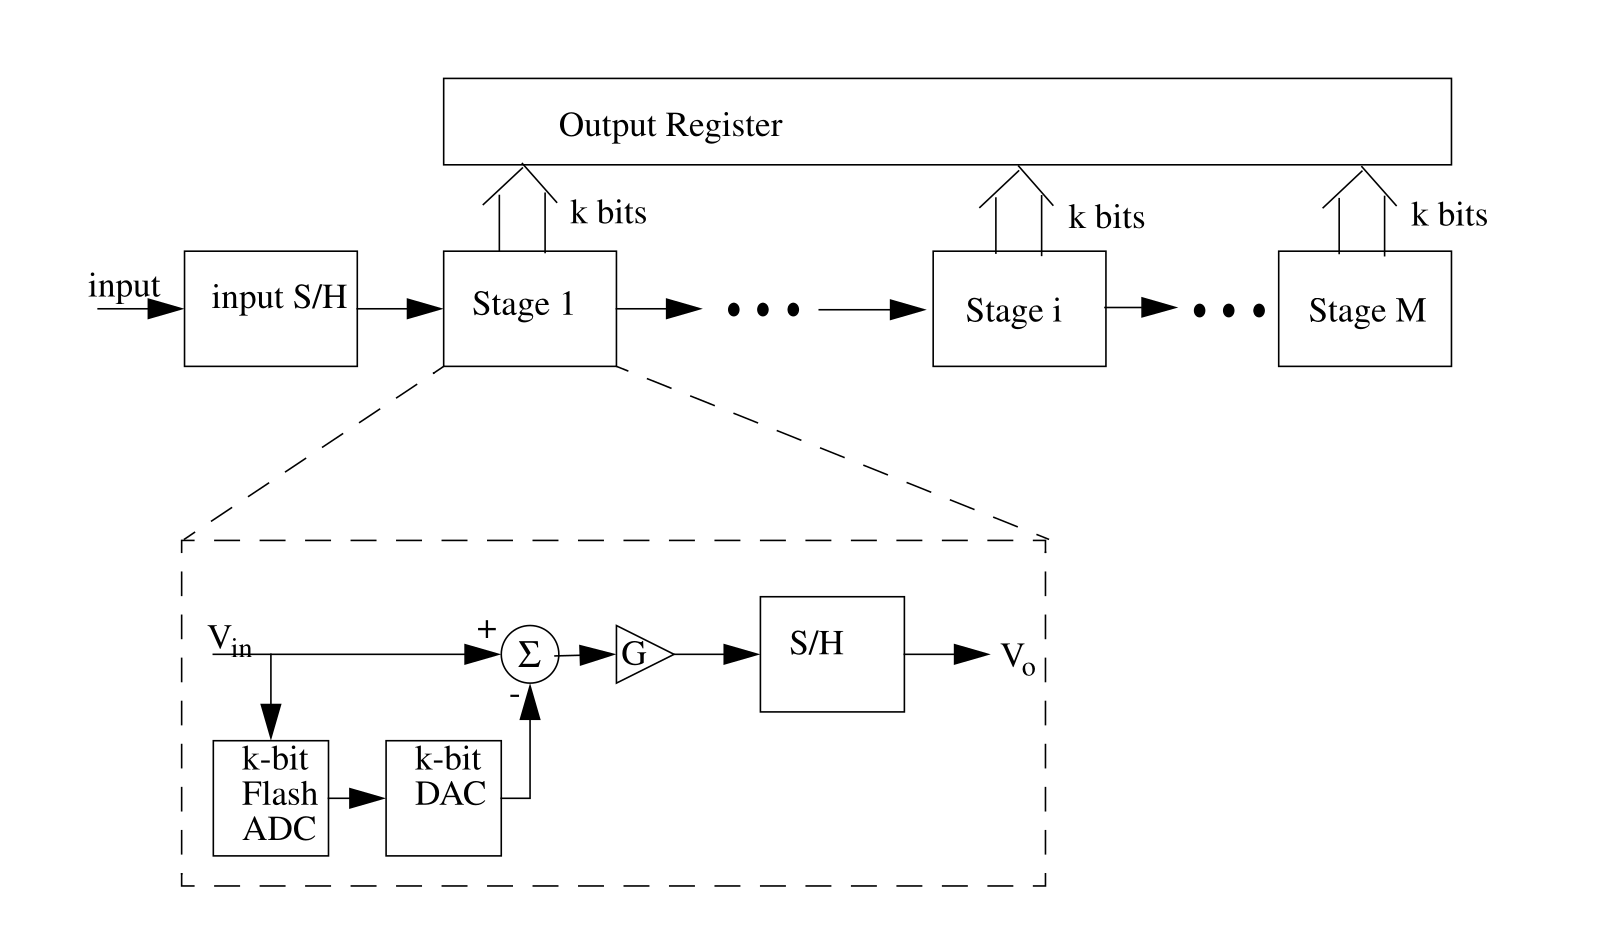
\includegraphics[width=\textwidth]{Pipeline_ADC.png}
    \caption{Иерархия разработки}
    \label{pic:ADC}
\end{figure}

На рисунке [insert] показана типичная конвейерная аналого-цифровая архитектура. Есть $M$ одинаковых каскадов, каждый квантует $k$ битов. Таким образом, общее разрешение $ M\dot k $. На каждом этапе производится выборка полученных данных из предыдущего этапа и квантование их до k-битных цифровых кодов с использованием архитектуры АЦП прямого преобразования. В Затем коды преобразуются в аналоговый сигнал с помощью k-битного ЦАП и вычитаются из дискретизированного сигнала. Затем остаток усиливается с коэффициентом усиления $ Av = 2^k $. Выходной регистр объединяет и  выводит биты с каждого каскада и дает окончательные цифровые коды. Этап 1 дает MSB, этап M дает младших битов. Чем позже этап, тем менее значимые биты он выводит из-за ограниченного коэффициента усиления на каждом этапе. Когда ступень завершает обработку выборки, определение битов и передачу остаточного сигнала на следующей ступени, он может затем начать обработку следующей выборки, полученной из устройства выборки и хранения. Это конвейерное действие является причиной высокой пропускной способности. \cite{pipelineADC}

Конвейерный аналого-цифровой преобразователь (АЦП) стал самой популярной архитектурой АЦП для частот дискретизации от нескольких мегасэмплов в секунду (Msps) до сотен мегасэмплов. Разрешающая способность варьируется от 8 бит при более высоких частотах дискретизации до 16 бит при более низких частотах. Эти разрешения и частоты дискретизации охватывают широкий спектр задач: формирование изображений CCD, ультразвуковая медицинская визуализацая, цифровые приемники, базовые станции, цифровое видео (например, HDTV), xDSL, кабельные модемы и Fast Ethernet. Приложения с более низкими частотами дискретизации по-прежнему являются областью поразрядных (SAR)  АЦП и интегрирующих архитектур, а в последнее время - АЦП с передискретизацией и сигма-дельта АЦП. Самые высокие частоты дискретизации (несколько сотен Msps или выше) по-прежнему достигаются с использованием АЦП прямого преобразования. Тем не менее, конвейерные АЦП различных форм в последние годы значительно улучшились по скорости, разрешающей способности, динамическим характеристикам и энергопотреблению.






Стоит отметить, что поскольку каждая выборка должна распространяться по всему конвейеру, прежде чем все связанные с ней биты станут доступными для объединения в части цифрового исправления ошибок, в конвейерном АЦП возникает задержка при передаче данных. В примере на рисунке [insert] эта задержка составляет около трех циклов [insert] . 


\paragraph{Цифровая калибровка}
Цифровая калибровка необходима для обеспечения превосходной точности и динамических характеристик АЦП. Для примера рассмотрим MAX1200 (16-bit, 1Msps). Он представляет собой КМОП-конвейерный АЦП с четырьмя 4-битными каскадами (с 1-битным перекрытием) и 5-битным АЦП прямого преобразования в конце. Дополнительные от одного до трех битов необходимы цифровой калибровке для квантования членов ошибки с большей точностью, чем сам АЦП; лишние биты также отбрасываются, чтобы получить в целом 14 или 16 бит. Калибровка начинается с MDAC на третьем этапе; после третьего этапа члены ошибки MDAC достаточно малы, поэтому калибровка не требуется. Выходной сигнал третьего каскада оцифровывается оставшимся конвейерным АЦП, а значения ошибок сохраняются во встроенной оперативной памяти. После калибровки третьего MDAC его можно использовать для калибровки второго и первого MDAC таким же способом. Для устранения шума используется усреднение. Во время нормального преобразования эти условия ошибок вызываются из ОЗУ и используются для настройки выходных сигналов логики цифрового исправления ошибок. 




\subsubsection{Сравнительный анализ конвейерного АЦП }


\section{Компаратор}

\subsection{Обзор компаратора}

Один из основных компонентов конвейерного АЦП, это АЦП прямого преобразования. Входное сравнение сигнала на последнем происходит при помощи компаратора. Таким образом, если не считать входное устройство выборки и хранения, то основное преобразование аналогового сигнала происходит именно в этой части, и его входной шум будет обеспечивать стохастическую ошибку, а также любые ошибки на уровне матчинга приборов будут приводить в систематическим ошибкам на уровне индивидуального устройства.
Для данного дизайна был выбран относительно классический дизайн компаратора на основе защелки из [insert]. Данный дизайн необходим для увеличения быстродействия системы без особого увеличения ее сложности или энергопотребления. Схема компаратора представлена на рисунке [insert]. Работает данная схема по принципу защелки.



\begin{figure}[H]
    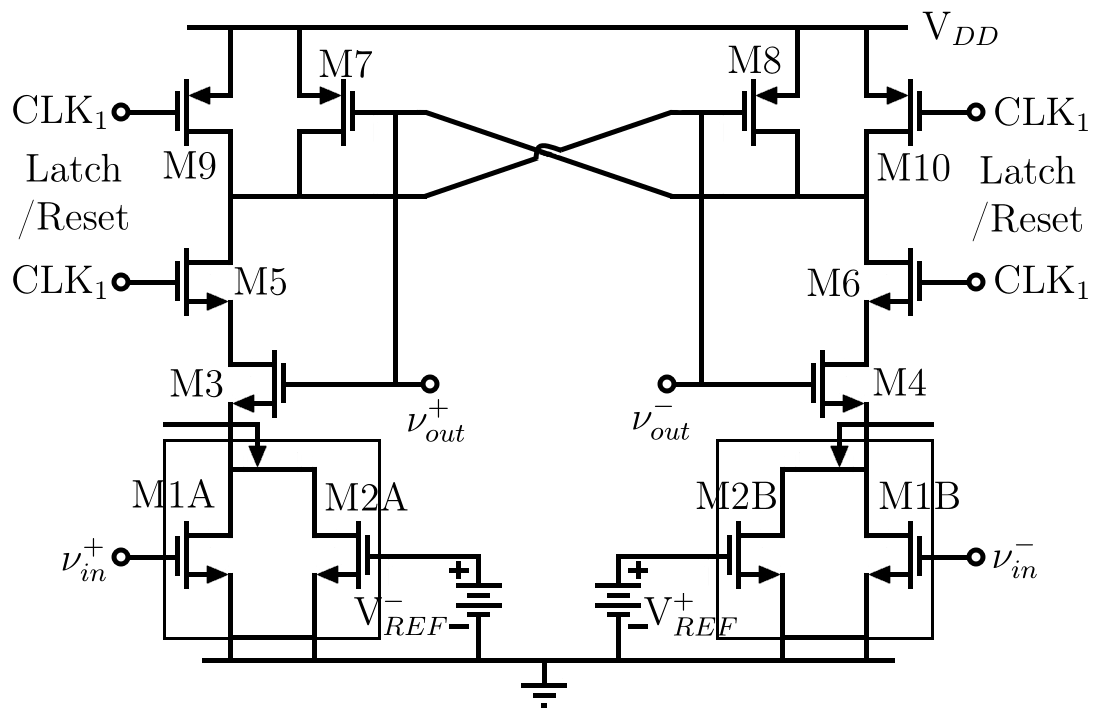
\includegraphics[width=\textwidth]{pre_comparator.png}
    \caption{Схема компаратора взятого за основу}
    \label{pic:pre_comparator}
\end{figure}

\begin{figure}[H]
    \begin{subfigure}[b]{0.45\textwidth}
      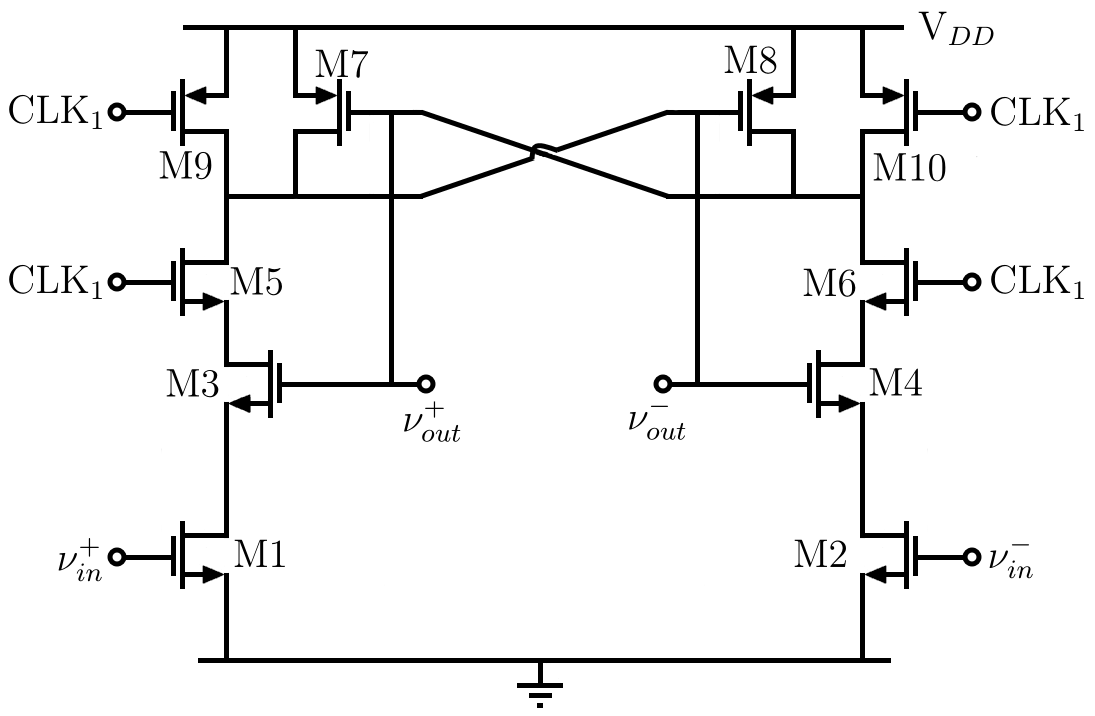
\includegraphics[width=\textwidth]{comparator_N}
      \caption{ N канальный вход }
      \label{pic:comparator_N}
    \end{subfigure}
    %
    \begin{subfigure}[b]{0.45\textwidth}
      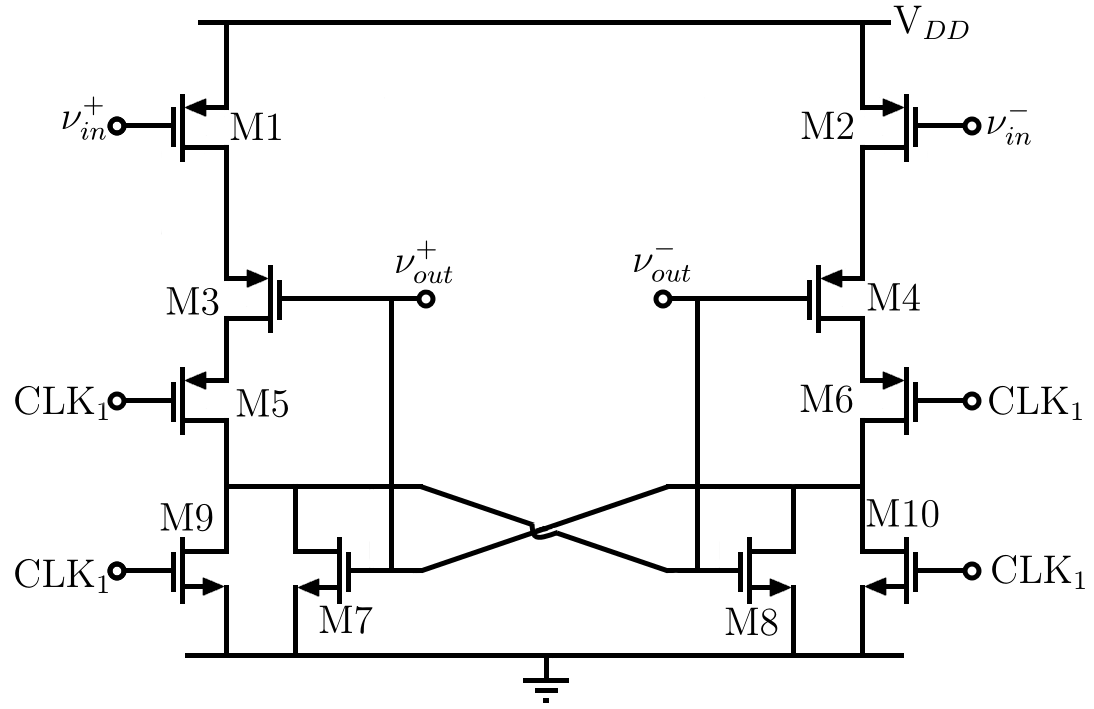
\includegraphics[width=\textwidth]{comparator}
      \caption{ P канальный вход (используется в АЦП в итоге) }
      \label{pic:comparator}
    \end{subfigure}
    \caption{Итоговая схема компаратора}
  \end{figure}



  Практический компаратор с защелкой показан на рис. [insert]. M7 и M8 - транзисторы формирующие защелку и, в данном случае, являющиеся PMOS. M9 и M10 используются для сброса защелки путем установки напряжения сток-исток M7 и M8 на ноль. Входной сигнал защелки подается на затворы MIA и MIB. Транзисторы M1A, MIB, M2A и M2B работают в области линейной области. Значения входов будут вызывать изменение сопротивления, видимого источниками M3 и M4 относительно земли. Когда защелка включена (в данном случае CLK HIGH)), стоки M3 и M4 подключаются к  выходам защелки. M3 и M4 образуют положительную обратную связь для защелки. Например, сигнал на затворе M7 может проходить через M7 или может проходить через M3 (M5 - замкнутый переключатель).  Пути обратной связи M3 и M4 зависят от канального сопротивления  или дополнительного сопротивления, R или R2, соответственно. Если сопротивление мало, коэффициент усиления велик, и на этой стороне компаратора установится высокий уровень напряжения.  При CLK LOW защелка переходит в регенеративный режим.  Ток стока M5 и M6 регулируется для получения конечного состояния, определяемого несоответствием между сопротивлениями R и R2.  Эти сопротивления представлены как ; 



\begin{equation}
    \frac{1}{R} = K_N [ \frac{W_{ 1 A}}{L}(V_{in^+} - V_T) + \frac{W_{ 2 A }}{L}(V_{ref}^- - V_T) ]
\end{equation}


\begin{equation}
    \frac{1}{R} = K_N [ \frac{W_{ 1 B}}{L}(V_{in^+} - V_T) + \frac{W_{ 2 B }}{L}(V_{ref}^+ - V_T) ]
\end{equation}

Выражение приравнивающее сопротивления:

$$ v_{in} = ( \frac{W_2}{W_1}V_{ref}) $$



Упрощенная форма компаратора на рис.[insert] показана на рис. [insert] В этом фиксированном компараторе входные напряжения v и vi определяют токи в M3 и M4.  Чем больше ток, тем больше коэффициент обратной связи через M3 или M4.   

\subsection{Полученные результаты }


В итоге был разработан компаратор с входным P каскадом для сравнения сигналов с общим уровнем от 0 до 4 вольт. Со скоростью срабатывания в приемлемые 4-5 нс. Компаратор потребляет примерно $50uA$ в момент сравнения, и не потребляет ток в остальное время. Таким образом, округляя вверх, можно сказать, что компаратор потребляет менее  $125$ мкрВт при  напряжении питания 5В.








\section{Операционный дифференциальный усилитель}

Операционные усилители (ОУ) являются важными компонентами аналоговой системы. Дизайн интегральной схемы часто использует операционные усилители для различных задач, таких как фильтры, регуляторы и функциональные генераторы, а также используется для создания буферов, логарифмических усилителей и инструментальных усилителей. В данной работе операционный усилитель с обратной связью на переключаемых конденсаторах используется для преобразования сигнала между ступенями MDAC. Операционные усилители также могут работать как простые компараторы, но для этой задачи был использован отдельный высокоскоростной компаратор. В данной работе были использованы в тои числе простые операционные усилители миллера, но они не представляют исследовательского или инженерного интереса.  Для прохождения сигнала между двумя ступенями ступенчатого АЦП, его нужно усилить на очень большой частоте и в режиме работы с очень глубокой обратной связью. То есть в десятки раз без потери в точности, но на частоте работы цифровой логики (в нашем случае 100МГц).


 В ходе разработки концепции был изучен целый ряд дизайнов [insert]. Выбранный  дизайн черпает вдохновение из целого ряда источников [insert]. Сам выбор сложенного каскада является типичным для подобных АЦП, поскольку подразумевает относительно малый выходной импеданс, а также широкие возможности по наращиванию усиления.  




\subsection{Сравнительный анализ различных видов ОУ}


\subsubsection{ОУ миллера}

Операционный усилитель миллера является самым классическим операционным усилителем применяемым в очень разных условиях, однако обладает рядом недостатков. Точнее сказать что его устройство слишком примитивно, чтобы позволять развивать его для получения характеристик сильно отличающихся друг от друга. Например, увеличение рабочей частоты неизменно ведет к очень сильному увеличению энергопотребления, а так же уменьшению коэффициента усиления. Таким образом при необходимости получить простой усилитель с характеристиками изменяющимимся при вариациях, а так же 


\subsubsection{Многоступенчатый каскодный усилитель}

Конструкция многоступенчатого усилителя всегда была важной темой исследований. Поскольку размеры устройств уменьшаются, напряжение питания становится ниже, а коэффициент усиления на каскад уменьшается. Топология каскода не подходит для низкого напряжения. Для достижения достаточного усиления по постоянному току необходимо использовать многокаскадные усилители. Многокаскадные усилители могут быть очень энергоэффективными при управлении большой емкостной нагрузкой, а некоторые даже достигают лучшей полосы пропускания, чем у однокаскадных усилителей \cite{op_amp_comp1}, \cite{op_amp_comp2}. Различные аналоговые устройства, например, линейные регуляторы с малым падением напряжения (LDR) и  драйверы матриц LCD, могут быть смоделированы как многокаскадные усилители, управляющие большой емкостной нагрузкой. Многие методы, разработанные для многокаскадных усилителей, такие как частотная компенсация с контролем добротности (DFCFC) [1] и активная частотная компенсация обратной связи (AFFC) \cite{op_amp_comp1}, находят применение в конструкциях OCF LDR \cite{op_amp_comp3}, \cite{op_amp_comp4}, и в нашем случае, в усилителе в АЦП. Несмотря на полезность многокаскадных усилителей, они страдают от проблем со стабильностью. Трехкаскадный усилитель имеет не менее трех узлов с высоким импедансом, каждый из которых вносит полюс. Плохая конструкция может легко привести к тому, что эти полюса будут работать с низкой частотой и вызвать проблемы со стабильностью. Также были разработаны различные методы частотной компенсации для обеспечения устойчивости системы \cite{op_amp_comp2}, \cite{op_amp_comp3}, \cite{op_amp_comp4} - \cite{op_amp_comp1}. Большинство этих структур являются производными от вложенной структуры компенсации Миллера (NMC) [14], которая использует простую компенсацию Миллера как во внутреннем, так и во внешнем компенсационном цикле. Внутренний конденсатор Миллера исключен в\cite{op_amp_comp1},\cite{op_amp_comp3},\cite{op_amp_comp4} и \cite{op_amp_comp2} . В [2], [9] - [11] простая компенсация Миллера во внешнем компенсационном контуре заменена более продвинутыми методами компенсации, такими как каскадная компенсация Миллера и компенсация Миллера текущего буфера. Многие из этих конструкций страдают от ограниченной комплексной полюсной частоты и большой добротности. В этой работе мы устраняем внутренний конденсатор Миллера и используем каскадную компенсацию Миллера [15] во внешнем компенсационном контуре для увеличения, и используем локальный блок ослабления импеданса (LIA), который состоит из серии RC сеть на выходе второй ступени [8] для управления сложными полюсами. Дизайн предлагаемого каскадного ослабления местного импеданса (CLIA)  позволяет достичь оптимального компромисса между резонансной частотой и добротностью. Остальная часть статьи организована следующим образом: в разделе В [insert] я определяю основную проблему конструкции трехкаскадного усилителя и предлагаю метод решения этой проблемы; в разделе [insert] обсуждаю структуру, конструктивные особенности и реализацию предложенного дизайна; в разделе [insert] мы показываем результаты измерений вместе с соответствующими обсуждениями; в разделе V мы завершаем проектные работы.


\paragraph{Компенсация}

За счет высокоомной ступени на выходе каждого каскада,  трехкаскадный усилитель имеет не менее трех полюсов. Для обеспечения стабильности методы компенсации перераспределяют положения полюсов. Простая компенсация Миллера  подключают компенсационный конденсатор между выходами первого и заключительной ступени для формирования внешнего компенсационного цикла. В некоторых схемах \cite{op_amp_comp5}, \cite{op_amp_comp6}, \cite{op_amp_comp7} к формированию двухтактный выходной каскад для улучшения переходных характеристик или создавать нули в левой полуплоскости для улучшения рабочей частоты. Таким образом, частота с единичным усилением (UGF) трехкаскадного усилителя зависит от расположения неосновных полюсов и наличие нулей левых полуплоскостей. Желательно подтолкнуть неосновные полюса к высокой частоте или компенсировать их нулями в левой полуплоскости, чтобы достичь высокой частоты единичного усиления. Во  дизайнах конструкциях недоминантные полюса представляют собой сложные полюса и совмещение  полюсов с нулями обычно невозможно. Таким образом, ключом к увеличению частоты единичного усиления является контроль сложных полюсов, то есть увеличение частоты этих полюсов и уменьшение добротности. Тем не менее они обычно взаимосвязаны и не могут контролироваться независимо. Снижение коэффициента добротности  обычно сопровождается сокращением также сокращением рабочей частоты, и это проблема - удовлетворить противоречивые требования увеличения частоты и усиления и снижения добротности. Оптимизированное комплексное управление полюсами схема должна сохранять низкую добротность, но сохранять  высокую частоту и усиление. Он также должен быть экономичным по площади и энергоэффективности, а также устойчивы к обработке вариаций по техпроцессу. Так же не создавать избыточную нагрузку на усилитель. В следующих параграфах мы кратко рассмотрим некоторые предыдущие методы управления сложными полюсами. 


Самый ранний и самый простой метод компенсации, это метод компенсации Миллера (Nested Miller compensation (NMC)).



\subsection{Изучение предложенной схемы устройства.}



\subsubsection{Стабильность}

Важным аспектом операционного усилителя с обратной связью является его устойчивость и невозможность перехода в режим осциллятора. Попробуем применить некоторые решения для увеличения устойчивости. Каков же критерий разрешения уравнения передаточной функции так, чтобы все полюса находились в левой части плоскости лапласа.

Причем в реалистичных сценариях нестабильность не возрастает до появления цепи обратной связи, с которой в нашем случае и планируется использовать усилитель.

Один из способов анализа линейной стационарной динамической системы на устойчивость, это критерий Гурвица [insert].


\subsection{Анализ слабого сигнала }

\begin{figure}[H]
    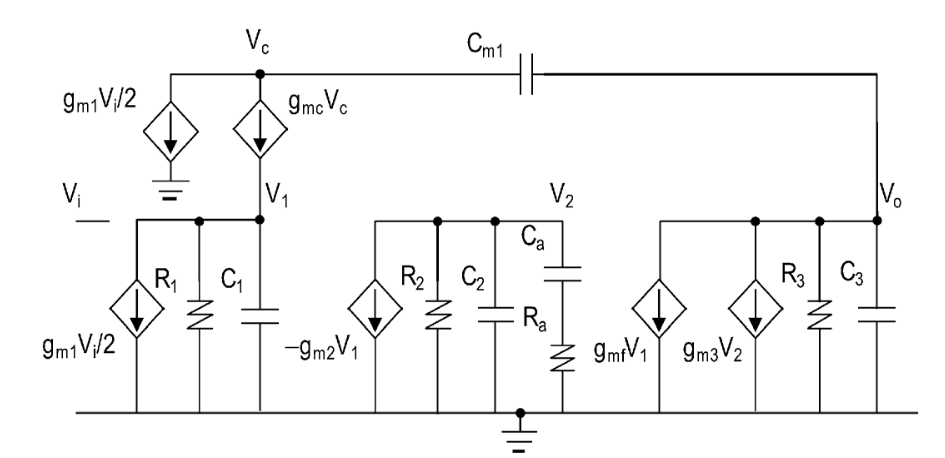
\includegraphics[width=\textwidth]{small_signal.png}
    \caption{Анализ слабого сигнала предложенного усилителя}
    \label{pic:small_signal}
\end{figure}

На \ref{pic:small_signal} показана эквивалентная слабосигнальная  схема разработанного   устройства. поставленный дизайн. Параметры $g_{mi}$, $ R_i $ , а также $ C_i $ это проводимость, выходное сопротивление и выходная емкость $i$ й ступени усилителя. Отметим, что $C_3$ включает оба паразитных конденсатора на последней ступени и конденсатор нагрузки . Используются следующие факты для упрощения вывода функции усиления. 
1) Поэтапное усиление каждого этапа намного больше чем один. 2) Компенсационный конденсатор , конденсатор LIA и конденсатор последней ступени намного больше, чем  емкости $ C_1 $ и $ C_2 $ . Тогда функция усиления предлагаемого усилителя определяется выражением:


$$ \frac{v_{o}}{v_{i}}\approx\frac{A_{DC}\left(1+\frac{s}{z_{1}}\right)\left(1+\frac{s}{z_{2}}\right)}{\left(1+\frac{s}{p_{0}}\right)\left(1+\frac{s}{p_{1}}\right)\left(1+\frac{1}{Q}\frac{s}{\omega_{o}}+\frac{s^{2}}{\omega_{o}}\right)}=\frac{g_{m1}g_{m2}g_{m3}R_{1}R_{2}R_{3}\left(1+sR_{a}C_{a}\right)}{\left(1+sg_{m2}g_{m3}R_{1}R_{2}R_{3}C_{m1}\right)\left(1+skR_{a}C_{a}\right)}\times $$ 

$$ \times  \frac{\left(1+\frac{sC_{m1}}{2g_{mc}}\right)}{\left(1 + \frac{sC_{1}C_{3}}{kg_{m2}g_{m3}R_{a}C_{m1}} + \frac{s^{2}C_{1}C_{3}}{kg_{m2}g_{m3}g_{mc}R_{a}}\right)}\; $$


где $k$ это:

$$k = 1 + \frac{C_{3}}{g_{m2}g_{m3}R_{1}R_{a}C_{m1}}\approx1.\;$$

Полюса $p_1$  и $p_2$ можно опредилить как:

$$p_{1} = \frac{1}{kR_{a}C_{a}}\;$$

$$z_{1} = \frac{1}{R_{a}C_{a}}.\;$$

После отмены полюсов ( $ -p_1 $ и  $  -z_1 $ к примеру), получаем:

$$\frac{v_{o}}{v_{i}}\approx\frac{g_{m1}g_{m2}g_{m3}R_{1}R_{2}R_{3}}{\left(1+sg_{m2}g_{m3}R_{1}R_{2}R_{3}C_{m1}\right)}\times\frac{\left(1+\frac{sC_{m1}}{2g_{mc}}\right)}{\left(1 + \frac{sC_{1}C_{3}}{g_{m2}g_{m3}R_{a}C_{m1}} + \frac{s^{2}C_{1}C_{3}}{g_{m2}g_{m3}g_{mc}R_{a}}\right)}.\;$$

Главный полюс определяющий усиление по постоянному току ($ -p_0 $ ) вычисляется как:

\subsection{Результаты работы усилителя без обратной связи}


\subsubsection{Частотные характеристики}



\subsubsection{Сравнение с другими работами}

\begin{table}[h]
    \begin{tabular}{|l|l|l|l|l|l|l|l|}
    \hline
                                                                                              & Эта работа               & \cite{op_amp_1}            & \cite{op_amp_2}           & \cite{op_amp_3}           & \cite{op_amp_4}         & \cite{op_amp_5}           & \cite{op_amp_6}         \\ \hline
    \begin{tabular}[c]{@{}l@{}}Усиление\\ (DC gain)\\  dB\end{tabular}                        & 66.0206                  & \textgreater{}100dB       & 72.04dB                  & 84dB                     & \textgreater{}100dB    & \textgreater{}100dB      & 67.81 dB               \\ \hline
    \begin{tabular}[c]{@{}l@{}}Полоса\\  единичного\\  усиления\\  (UGF),\\  MHZ\end{tabular} & 700                      & 3.49                      & 13.33                    & 0.013                    &                        & 2                        & 0.9643                 \\ \hline
    Нагрузка                                                                                  & 0.1p                     & 560pF                     & 2pF                      & 15nF                     & 500pF                  & 500pF                    & -                      \\ \hline
    \begin{tabular}[c]{@{}l@{}}Ток\\  потребления\\  основным \\ каскадом,\\  uA\end{tabular} & \multicolumn{1}{r|}{90}  & \multicolumn{1}{r|}{10.5} & -                        & \multicolumn{1}{r|}{3}   & \multicolumn{1}{r|}{7} & \multicolumn{1}{r|}{17}  & -                      \\ \hline
    \begin{tabular}[c]{@{}l@{}}Напряжение\\  питания,\\ V\end{tabular}                        & \multicolumn{1}{r|}{5}   & \multicolumn{1}{r|}{1.2}  & \multicolumn{1}{r|}{1.8} & \multicolumn{1}{r|}{1.2} & 0.9                    & \multicolumn{1}{r|}{1.2} & \multicolumn{1}{r|}{1} \\ \hline
    Мощность                                                                                  & \multicolumn{1}{c|}{1mW} & 12.7uW                    & <0.13mW                  & 3.6uW                    & 6.3uW                  & 20.4uW                   & 724uW                  \\ \hline
    Технология                                                                                & 0.18u SOI                & 0.13um                    & 0.18um                   & 0.18um                   & 0.18um                 & 65nm                     & 0.18um                 \\ \hline
    \end{tabular}
    \caption{Сравнение с другими работами по операционным усилителям}
    \label{tab:op_amp_comp}
    \end{table}





\subsection{Обратная связь операционного усилителя}



\begin{figure}[H]
    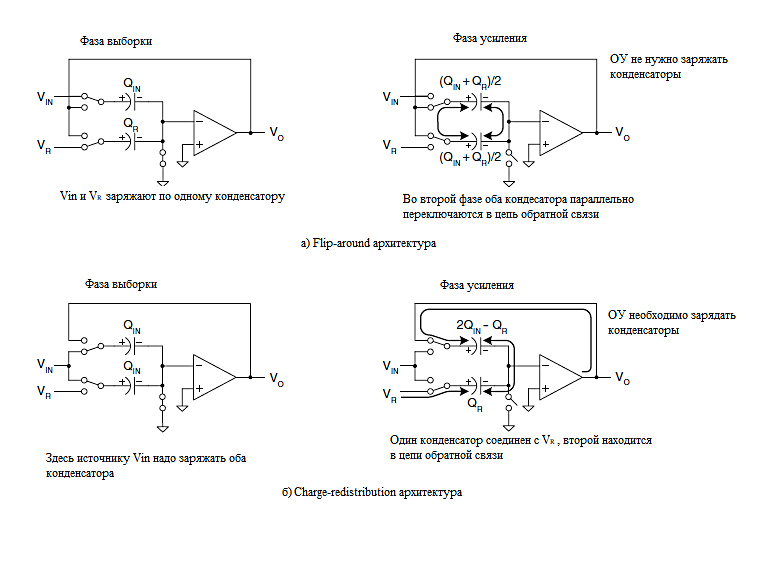
\includegraphics[width=\textwidth]{Dve_arkhitektury.jpg}
    \caption{Две самые популярные архитектуры обратной связи}
    \label{pic:feedback}
\end{figure}



В нашем случае использование резистивной обратной связи исключено из соображений быстродействия и качества изготавливаемых в техпроцессе резисторов. Используется же обратная связь на переключаемых конденсаторах. 
Суть такой обратной связи та же что и у резистивной: получить усиление независимоcти от процессных  и температурных вариаций, увеличение скорости, уменьшение энергопотребления. Резистивная же обратная связь попросту не может обеспечить требуемых характеристик учитывая ограниченность резисторов на кристалле и их огромную вариацию. 

Существует несколько видов м
Конкретно используется “flip-around” архитектура. Также известная как архитектура переворота заряда.
Преимущества “flip-around” архитектуры. Архитектура потребляет меньше мощности, чем архитектура перераспределения заряда используется в обычных MDAC по двум причинам. Во-первых, усилитель не должен заряжать конденсаторы во время фазы удержания. Как показано на рисунке [insert], в архитектуре с переворотом дискретный заряд распределяется только между двумя конденсаторами во время фазы удержания. Однако в архитектуре перераспределения заряда усилитель заряжает конденсаторы, потому, что выбранный заряд перераспределяется между двумя конденсаторами во время фазы ожидания. Поэтому усилитель с обратной связью на архитектуре перевернутого типа потребляет меньше энергии, чем усилитель архитектуры перераспределения заряда. Во-вторых, конденсатор подключены к входным и выходным узлам усилителя только во время фазы удержания. Следовательно, коэффициент обратной связи от выходного узла к входному узлу усилителя равен 1. В отличие от архитектуры перераспределения заряда, вход усилителя - средний узел из двух последовательных конденсаторы, поэтому коэффициент усиления обратной связи равен 0,5. Усиление обратной связи влияет на скорость работы во время Фаза удержания: чем ниже усиление обратной связи, тем больше время установления. Когда ширина полосы пропускания произведение усилителя фиксировано, время установления во время фазы удержания с переворотом короче, чем с архитектурой распределения заряда, потому что обратная связь в два раза выше. Другими словами, Требования по произведению ширины полосы пропускания ослаблены, что означает, что требуется меньшая мощность, чтобы добиться желаемого времени установления во время фазы удержания.






\section{PVT источник тока}


Для работы компонентов аналоговой электроники, в нашем случае операционных усилителей, критично иметь не только источник напряжения, но и стабильный источник тока. Источник тока как рассмотрено выше является критическим компонентом для усилителей используемых в АЦП. Стабильность источника определяется стабильностью генерации опорного тока по отношению к трем варьируемым параметрам: напряжению питания, температурой и процессным вариациям\cite{op_amp_comp10}. Небольшие отклонения в колебаниях питающего напряжения или тока могут приводить к значительным колебаниям в значениях генерируемого тока у простых источников на подобии резистора.  Так же нужно держать во внимании просцессные вариации (отклонения заданных  значений компонентов от желаемых) которые могут быть очень значительными у тех же резисторов для КМОП техпроцессов. Остается только генерировать напряжение на основе фиксированных физических величин. Классические дизайны температурно устойчивых источников подразумевают схемы на основе биполярных транзисторов, которых нет в предлагаемом КНИ техпроцессе. Был выбран источник тока на основе порогового напряжения КМОП транзистора (Threshold voltage)\cite{op_amp_comp11}. Данное значение не сильно изменяется от температуры и вариаций длинны и ширины и вообще не зависит от напряжения питания, изменяясь лишь от эффекта плавающего напряжения (body effect) [insert]. Типичная цепь генерации тока на основе порогового напряжения выглядит как [insert]. В ходе симуляции отдельно учитывая T или V вариации удалось измерить, что отклонения тока от заданного менее 1\% при варьировании температуры в переделах от -20 до 80 градусов. И менее 1\% вариировании напряжения от 4.5V до 5.5V. Попробуем описать ее устройство, а потом перейдем к полученным результатам.


\subsection{Описание устройства Источника тока }


Далее я опишу устройство выбранного источника. Его приблизительная схема представлена на рисунке [insert].
Для начала M3 и M4 уравнивают ток $ I_1 $ и $ I_2 $. Ток $I_1$ через M1 генерирует напряжение $V_{gs1}$, а $I_2$ создает напряжение $I_2 R $ . Поскольку эти два напряжения связаны между собой, то, когда цепь стабильна\cite{op_amp_comp12}. На рисунке 1.2 показан метод определения устойчивой рабочей  точки как пересечения двух характеристик. 
 На кривой $ I_1 $ и $ I_2 $ представлены как функция напряжения. Пересечение этих кривых определяет рабочую точку $Q$. Уравнение равновесия описывается так: 

 $$ I_2 R = v_{T1} + ( \frac{2I_1 L_1}{ K_N W_1})^{\frac{1}{2}} $$

 Поскольку из за описаных выше условий $ I1=I2=IQ $, мы можем разрешить это (игнорируя короткоканальные эффекты) как:

\begin{equation}
    I_Q = I_2 =  \frac{V_T1}{R} + \frac{1}{\beta_1 R^2} + \frac{1}{R} \sqrt{ \frac{2 V_{T1}}{\beta_1 R} + \frac{1}{\beta_1^2 R^2}}
\end{equation}

Откуда видно что $I_1$ и $I_2$ не меняются в первом приближении от колебаний напряжения, так что чувствительность к колебаниям напряжения уменьшается. 


К сожалению, как видно из нее, у данной цепи возможно два устойчивых состояния, нужное нам, и то в котором ток через цепь не течет. Поэтому данной схеме необходима пусковая цепь\cite{op_amp_comp13}. Схема вместе с пусковой схемой представлена на  [insert]. Значения ширин транзисторов представлены в таблице [insert]. 

\subsubsection{Итоговая схема и ее анализ}

Итоговая схема источника тока с учетом температуры и вариации по напряжению представлена на рисунке [insert]. 







\subsubsection{Результаты работы источника}


В этой главе я представлю результаты реботы источника тока по вариациям напряжения, процессов производства и температуре.





\begin{figure}[H]
    \begin{subfigure}[b]{0.5\textwidth}
      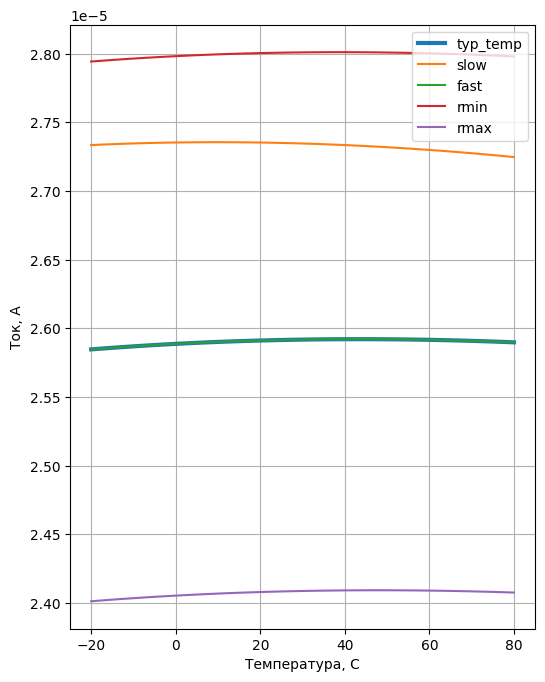
\includegraphics[width=\textwidth]{current_temp_thin.png}
      \caption{ Вариация по температуре }
      \label{pic:current_temp_thin}
    \end{subfigure}
    %
    \begin{subfigure}[b]{0.5\textwidth}
      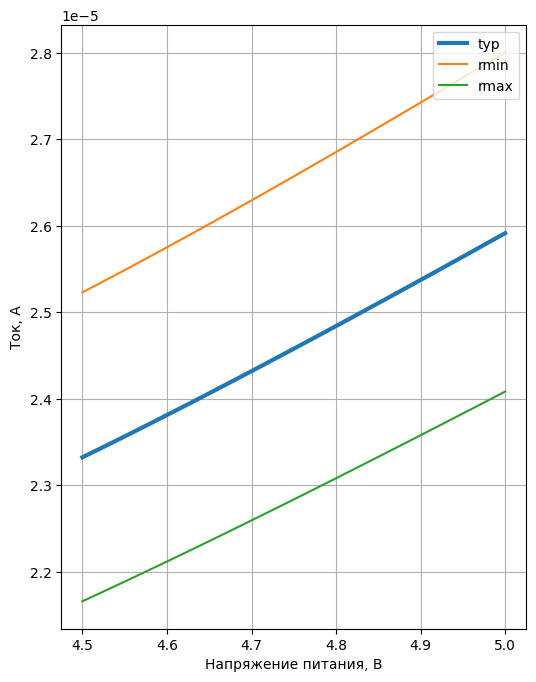
\includegraphics[width=\textwidth]{current_vdd_thin.png}
      \caption{ Вариация по напряжению питания }
      \label{pic:current_vdd_thin}
    \end{subfigure}
    \caption{Графики вариаций}
  \end{figure}


  \begin{figure}[H]
    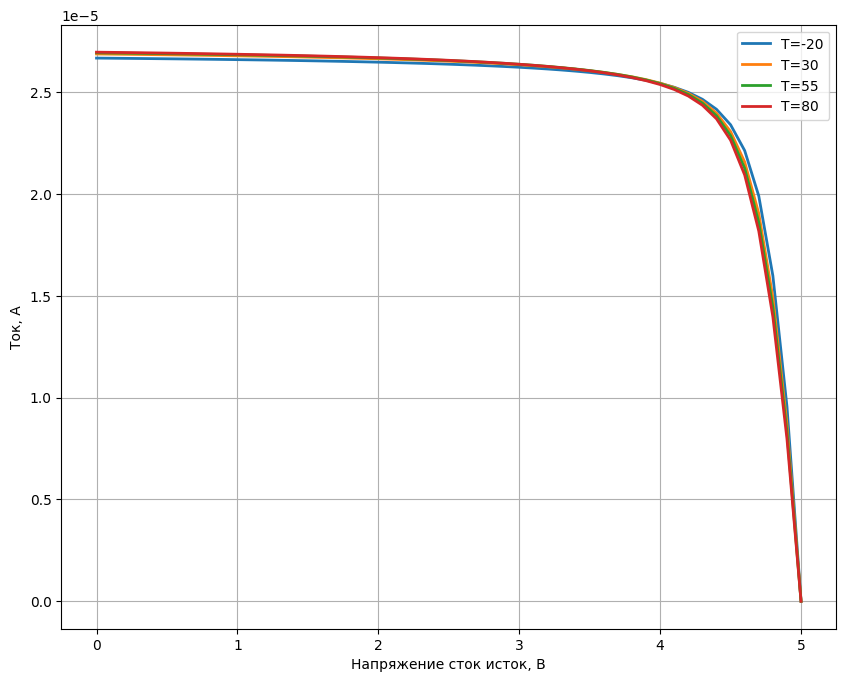
\includegraphics[width=\textwidth]{temp_vds.png}
    \caption{Характеристика транзистора в зависимости от температуры}
    \label{pic:new}
\end{figure}



\subsection{Выводы}




\begin{thebibliography}{}
\bibitem{Segneto_MIPT-I}  Improved Ferroelectric Switching Endurance of La-Doped $Hf_{0.5}Zr_{0.5}O_2$
Thin Films
Anna G. Chernikova, Maxim G. Kozodaev, Dmitry V. Negrov, Evgeny V. Korostylev,
Min Hyuk Park, Uwe Schroeder, Andrey M. Markeev,

\bibitem {FRAM} Advanced Circuit Design of
Gigabit-Density Ferroelectric
Random-Access Memories Jürgen Thomas Rickes aus Neuwied  


\bibitem{pipelineADC} Design Techniques for Parallel Pipelined ADC  by Li Lin
\bibitem{op_amp_1}	S. Guo and H. Lee, “Dual active-capacitive-feedback compensation	
\bibitem{op_amp_2}	"Design of High PSRR Folded Cascode Operational Amplifier for LDO Applications
Harsh Gupta, Gaurav Kumar Mishra, Mr. Navaid Zafar Rizvi, and Dr. Santosh Kumar Patnaik"	
\bibitem{op_amp_3} 	Z. Yan, P.-I. Mak, M.-K. Law, R. Martins, and F. Maloberti, “A 0.0013mm3.6W nested-current-mirror single-stage amplifier driving0.15-to-15 nF capacitive loads withphase margin,”
\bibitem{op_amp_4}	W. Qu, J.-P. Im, H.-S. Kim, and G.-H. Cho, “A 0.9 V 6.3multi-stage amplifier driving 500 pF capacitive load with 1.34 MHz GBW,”	
\bibitem{op_amp_5}	S. S. Chong and P. K. Chan, “Cross feedforward cascode compensationfor low-power three-stage amplifier with large capacitive load,”	
\bibitem{op_amp_6}	Raghav,  H.S.,  Singh,  B.P.,  Maheshwari.  S,  “Design  of  Low  Voltage  OTA  for  Bio-medical  Application,” 	


\bibitem{op_amp_comp1} K. N. Leung, P. K. T. Mok, W. H. Ki, and J. K. O. Sin, “Three-stage
large capacitive load amplifier with damping-factor-control frequency
compensation,” IEEE J. Solid-State Circuits, vol. 35, no. 2, pp.
221–230, Feb. 2000.
\bibitem{op_amp_comp2} H. Lee and P. K. T. Mok, “Active-feedback frequency-compensation
technique for low-power multistage amplifiers,” IEEE J. Solid-State
Circuits, vol. 38, no. 3, pp. 511–520, Mar. 2003.
\bibitem{op_amp_comp3} K. N. Leung and P. K. T. Mok, “A capacitor-free CMOS low-dropout
regulator with damping-factor-control frequency compensation,” IEEE
J. Solid-State Circuits, vol. 38, no. 10, pp. 1691–1702, Oct. 2003.
\bibitem{op_amp_comp4} E. N. Y. Ho and P. K. T. Mok, “A capacitor-less CMOS active feedback
low-dropout regulator with slew-rate enhancement for portable on-chip
application,” IEEE Trans. Circuits Syst. II, Exp. Briefs, vol. 57, no. 2,
pp. 80–84, Feb. 2010.
\bibitem{op_amp_comp5} X. Peng and W. Sansen, “AC boosting compensation scheme for low-
power multistage amplifiers,” IEEE J. Solid-State Circuits, vol. 39, no.
11, pp. 2074–2079, Nov. 2004.

\bibitem{op_amp_comp6} A. D. Grasso, G. Palumbo, and S. Pennisi, “Advances in reversed
nested Miller compensation,” IEEE Trans. Circuits Syst. I, Reg.
Papers, vol. 54, no. 7, pp. 1459–1470, Jul. 2007.
\bibitem{op_amp_comp7} X. Peng, W. Sansen, L. Hou, J. Wang, and W. Wu, “Impedance adapting compensation for low-power multistage amplifiers,” IEEE J. Solid-State Circuits, vol. 46, no. 2, pp. 445–451, Feb. 2011.
\bibitem{op_amp_comp8} S. Guo and H. Lee, “Dual active-capacitive-feedback compensation
for low-power large-capacitive-load three-stage amplifiers,” IEEE J.
Solid-State Circuits, vol. 46, no. 2, pp. 452–464, Feb. 2011.
\bibitem{op_amp_comp9} S. S. Chong and P. K. Chan, “Cross feedforward cascode compensation
for low-power three-stage amplifier with large capacitive load,” IEEE
J. Solid-State Circuits, vol. 47, no. 9, pp. 2227–2234, Sep. 2012.
\bibitem{op_amp_comp10} Design and Simulation of a CMOS Current Source Cell
Kaiyu Wangaa, Zhenan Tang, Hualong Li, Yun Zhao, Xi Song,
Jiandong Su.
\bibitem{op_amp_comp11} Phillip E Allen, Douglas R Holberg. CMOS Analog Circuit Design, 2nd Edition. Oxford:Oxford University Press, 2002.
\bibitem{op_amp_comp12}Alan Hastings .The Art of Analog Layout Second Edition. Prentice Hall Press,2005.
\bibitem{op_amp_comp13}Razavi B.Design of Analog CMOS Integrated Circuits[M]Boston,MA:McGraw-Hill Press,2001.

\end{thebibliography}



\end{document}
